%%%%%%%%%%%%%%%%%%%%%%%%%%%%%%%%%%%%%%%%%
% Short Sectioned Assignment
% LaTeX Template
% Version 1.0 (5/5/12)
%
% This template has been downloaded from:
% http://www.LaTeXTemplates.com
%
% Original author:
% Frits Wenneker (http://www.howtotex.com)
%
% License:
% CC BY-NC-SA 3.0 (http://creativecommons.org/licenses/by-nc-sa/3.0/)
%
%%%%%%%%%%%%%%%%%%%%%%%%%%%%%%%%%%%%%%%%%

%----------------------------------------------------------------------------------------
%	PACKAGES AND OTHER DOCUMENT CONFIGURATIONS
%----------------------------------------------------------------------------------------

\documentclass[paper=a4, fontsize=11pt]{scrartcl} % A4 paper and 11pt font size

\usepackage[T1]{fontenc} % Use 8-bit encoding that has 256 glyphs
\usepackage{fourier} % Use the Adobe Utopia font for the document - comment this line to return to the LaTeX default
\usepackage[spanish]{babel} % English language/hyphenation
\selectlanguage{spanish}
\usepackage[utf8]{inputenc}
\usepackage{amsmath,amsfonts,amsthm} % Math packages
\usepackage{graphicx}

\usepackage{sectsty} % Allows customizing section commands
\allsectionsfont{\centering \normalfont\scshape} % Make all sections centered, the default font and small caps

\usepackage{fancyhdr} % Custom headers and footers
\pagestyle{fancyplain} % Makes all pages in the document conform to the custom headers and footers
\date{}
\fancyhead{} % No page header - if you want one, create it in the same way as the footers below
\fancyfoot[L]{} % Empty left footer
\fancyfoot[C]{} % Empty center footer
\fancyfoot[R]{\thepage} % Page numbering for right footer
\renewcommand{\headrulewidth}{0pt} % Remove header underlines
\renewcommand{\footrulewidth}{0pt} % Remove footer underlines
\setlength{\headheight}{5.6pt} % Customize the height of the header

\numberwithin{equation}{section} % Number equations within sections (i.e. 1.1, 1.2, 2.1, 2.2 instead of 1, 2, 3, 4)
\numberwithin{figure}{section} % Number figures within sections (i.e. 1.1, 1.2, 2.1, 2.2 instead of 1, 2, 3, 4)
\numberwithin{table}{section} % Number tables within sections (i.e. 1.1, 1.2, 2.1, 2.2 instead of 1, 2, 3, 4)

\setlength\parindent{0pt} % Removes all indentation from paragraphs - comment this line for an assignment with lots of text

%----------------------------------------------------------------------------------------
%	TITLE SECTION
%----------------------------------------------------------------------------------------

\newcommand{\horrule}[1]{\rule{\linewidth}{#1}} % Create horizontal rule command with 1 argument of height

\title{	
\normalfont \normalsize 
\textsc{UNIVERSIDAD DE CANTABRIA, DEPARTAMENTO DE FÍSICA MODERNA} \\ [20pt] % Your university, school and/or department name(s)
\horrule{0.5pt} \\[0.4cm] % Thin top horizontal rule
\huge Física de Partículas Elementales (G71) \\ % The assignment title
\normalsize 4 Curso - Grado de Física
\horrule{2pt} \\[0.5cm] % Thick bottom horizontal rule
}

\begin{document}

\maketitle % Print the title

\vspace{-2.5cm}

%----------------------------------------------------------------------------------------
%	PROBLEM 1
%----------------------------------------------------------------------------------------
\textbf{Cuestión 1.} Un pion cargado colisiona con un protón en reposo dando lugar a un pion cargado, un protón y un pion neutro ($\pi^{+} + p^{+}\rightarrow\pi^{+}+p^{+}+\pi^{0}$). ¿Cuál es la energía mínima
del pion incidente para que esta reacción sea posible?. M($\pi^{+}$)=0.140~GeV, M($\pi^{0}$)=0.135~GeV, M($p^{+}$)=0.938~GeV. \textbf{(1 Punto)}. Demuestra que la reacción $e^{-}\rightarrow e^{-}+\gamma$ no
es posible en el vacío. \textbf{(1 Punto)}.
\\
\\
%----------------------------------------------------------------------------------------
%       PROBLEM 2
%----------------------------------------------------------------------------------------
\textbf{Cuestión 2.} Prueba las siguientes relaciones de las matrices $\gamma$ \textbf{(1 Punto)}: 
\begin{enumerate}
\item $\gamma_\mu\gamma^\mu=4I$
\item $\gamma_\mu\gamma_\nu a^{\nu}\gamma^{\mu}=-2\gamma_\nu a^{\nu}$
\item $\gamma_\mu\gamma_\nu a^{\nu}\gamma_\lambda b^{\lambda}\gamma^{\mu}=4 a_{\mu}b^{\mu}I$.
\end{enumerate}
Demuestra que cada una de las componentes de los espinores de Dirac cumple la ecuación de Klein-Gordon ($\partial_\mu\partial^{\mu} + m^2)\psi_i = 0$. Para ello multiplica a la ecuación de Dirac
por $(i\gamma^{\nu}\partial_{\nu} + m)$ y opera sabiendo que $\gamma^{\nu}\gamma^{\mu}a_{\mu}a_{\nu}=\frac{1}{2}(\gamma^{\nu}\gamma^{\mu} + \gamma^{\mu}\gamma^{\nu})a_{\mu}a_{\nu}$. \textbf{(1 Punto)}.
%----------------------------------------------------------------------------------------
\\
\\
%----------------------------------------------------------------------------------------
%       PROBLEM 3
%----------------------------------------------------------------------------------------
\textbf{Cuestión 3.} Considera el proceso de aniquilación $q^{-}q^{+}\rightarrow q^{-} q^{+}$. Dibuja los tres posibles diagramas de Feynmann de 2 vértices que contribuyen a este proceso. \textbf{(0.5 Puntos)}. Indica
la estructura que tendría el elemento de matriz asociado a cada uno de ellos, explicando las diferencias. \textbf{(1 Punto)}. Ordena los tres diagramas de mayor a menor sección eficaz en un experimento con
una energía del centro de masas de $\sqrt{10}~GeV$. Razona tu respuesta. \textbf{(0.5 Puntos)}.  
%----------------------------------------------------------------------------------------
\\
\\
%----------------------------------------------------------------------------------------
%       PROBLEM 4
%----------------------------------------------------------------------------------------
\textbf{Cuestión 4.} Definir el concepto de helicidad y de quiralidad. ¿Cuándo son coincidentes? \textbf{(0.5 Puntos)}. Define el concepto del operador conjugación de carga C y del operador de paridad P. ¿Cómo afecta
el operador C a los spinores de partícula y antipartícula canónicos? \textbf{(0.5 Puntos)}. Define los siguientes conceptos o magnitudes: tasa de transición, sección eficaz, sección eficaz diferencial, densidad de estados,
elemento de matriz. ¿Cuales de las magnitudes anteriores son invariantes Lorentz y cuáles no?. \textbf{(0.5 Puntos)}. Define qué entendemos por confinamiento del color y cómo se relaciona con el llamado proceso de
hadronización. \textbf{(0.5 Puntos)}.
\\
\\
%----------------------------------------------------------------------------------------
%       PROBLEM 5
%----------------------------------------------------------------------------------------
\textbf{Cuestión 5.} La desintegración del pion cargado resulta a priori sorprendente ya que se produce mayoritariamente en la forma ($\pi^{-}\rightarrow\mu^{-}\bar{\nu}$) y no de la forma ($\pi^{-}\rightarrow e^{-}\bar{\nu}$). Explica
por qué esto resulta sorprendente al menos desde un punto de vista meramente energético. \textbf{(0.5 Puntos)}. Asumiendo que un pion cargado negativamente está en reposo y sabiendo que su spin es nulo: dibuja esquemáticamente
cómo tendría lugar su desintegración a un leptón cargado y a un antineutrino señalando las direcciones y espines de las partículas involucradas. Considera todas las posibilidades a priori posibles. \textbf{(0.5 Puntos)}. 
Asumiendo que la masa del neutrino es exactamente cero, razona cuál de las opciones tendrá lugar en la naturaleza y demuestra matemáticamente que el cociente entre la tasa de desintegración a muones y a electrones 
debe ser proporcional a aproximadamente $m_{\mu}^2/m_{e}^2$. Utiliza para ello los espinores dados a continuación. \textbf{(1 Punto)}. 
  

\begin{figure}[!h]
\begin{center}
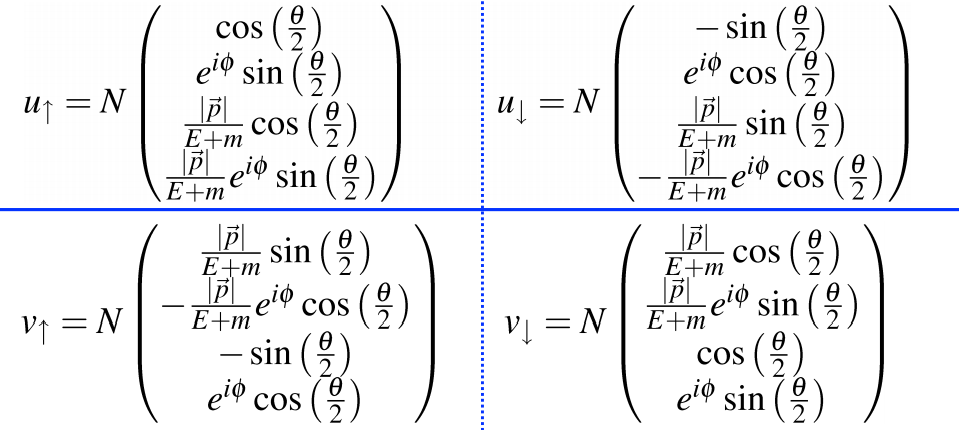
\includegraphics[width=0.6\linewidth]{espinores.png}
\end{center}
\caption{Espinores solución a la ecuación de Dirac y autoestados del operador helicidad.}
\label{espinores}
\end{figure}






\end{document}
